% Options for packages loaded elsewhere
\PassOptionsToPackage{unicode}{hyperref}
\PassOptionsToPackage{hyphens}{url}
%
\documentclass[
  man, donotrepeattitle,floatsintext]{apa6}
\usepackage{amsmath,amssymb}
\usepackage{lmodern}
\usepackage{iftex}
\ifPDFTeX
  \usepackage[T1]{fontenc}
  \usepackage[utf8]{inputenc}
  \usepackage{textcomp} % provide euro and other symbols
\else % if luatex or xetex
  \usepackage{unicode-math}
  \defaultfontfeatures{Scale=MatchLowercase}
  \defaultfontfeatures[\rmfamily]{Ligatures=TeX,Scale=1}
\fi
% Use upquote if available, for straight quotes in verbatim environments
\IfFileExists{upquote.sty}{\usepackage{upquote}}{}
\IfFileExists{microtype.sty}{% use microtype if available
  \usepackage[]{microtype}
  \UseMicrotypeSet[protrusion]{basicmath} % disable protrusion for tt fonts
}{}
\makeatletter
\@ifundefined{KOMAClassName}{% if non-KOMA class
  \IfFileExists{parskip.sty}{%
    \usepackage{parskip}
  }{% else
    \setlength{\parindent}{0pt}
    \setlength{\parskip}{6pt plus 2pt minus 1pt}}
}{% if KOMA class
  \KOMAoptions{parskip=half}}
\makeatother
\usepackage{xcolor}
\usepackage{graphicx}
\makeatletter
\def\maxwidth{\ifdim\Gin@nat@width>\linewidth\linewidth\else\Gin@nat@width\fi}
\def\maxheight{\ifdim\Gin@nat@height>\textheight\textheight\else\Gin@nat@height\fi}
\makeatother
% Scale images if necessary, so that they will not overflow the page
% margins by default, and it is still possible to overwrite the defaults
% using explicit options in \includegraphics[width, height, ...]{}
\setkeys{Gin}{width=\maxwidth,height=\maxheight,keepaspectratio}
% Set default figure placement to htbp
\makeatletter
\def\fps@figure{htbp}
\makeatother
\setlength{\emergencystretch}{3em} % prevent overfull lines
\providecommand{\tightlist}{%
  \setlength{\itemsep}{0pt}\setlength{\parskip}{0pt}}
\setcounter{secnumdepth}{-\maxdimen} % remove section numbering
% Make \paragraph and \subparagraph free-standing
\ifx\paragraph\undefined\else
  \let\oldparagraph\paragraph
  \renewcommand{\paragraph}[1]{\oldparagraph{#1}\mbox{}}
\fi
\ifx\subparagraph\undefined\else
  \let\oldsubparagraph\subparagraph
  \renewcommand{\subparagraph}[1]{\oldsubparagraph{#1}\mbox{}}
\fi
\newlength{\cslhangindent}
\setlength{\cslhangindent}{1.5em}
\newlength{\csllabelwidth}
\setlength{\csllabelwidth}{3em}
\newlength{\cslentryspacingunit} % times entry-spacing
\setlength{\cslentryspacingunit}{\parskip}
\newenvironment{CSLReferences}[2] % #1 hanging-ident, #2 entry spacing
 {% don't indent paragraphs
  \setlength{\parindent}{0pt}
  % turn on hanging indent if param 1 is 1
  \ifodd #1
  \let\oldpar\par
  \def\par{\hangindent=\cslhangindent\oldpar}
  \fi
  % set entry spacing
  \setlength{\parskip}{#2\cslentryspacingunit}
 }%
 {}
\usepackage{calc}
\newcommand{\CSLBlock}[1]{#1\hfill\break}
\newcommand{\CSLLeftMargin}[1]{\parbox[t]{\csllabelwidth}{#1}}
\newcommand{\CSLRightInline}[1]{\parbox[t]{\linewidth - \csllabelwidth}{#1}\break}
\newcommand{\CSLIndent}[1]{\hspace{\cslhangindent}#1}
\ifLuaTeX
\usepackage[bidi=basic]{babel}
\else
\usepackage[bidi=default]{babel}
\fi
\babelprovide[main,import]{english}
% get rid of language-specific shorthands (see #6817):
\let\LanguageShortHands\languageshorthands
\def\languageshorthands#1{}
% Manuscript styling
\usepackage{upgreek}
\captionsetup{font=singlespacing,justification=justified}

% Table formatting
\usepackage{longtable}
\usepackage{lscape}
% \usepackage[counterclockwise]{rotating}   % Landscape page setup for large tables
\usepackage{multirow}		% Table styling
\usepackage{tabularx}		% Control Column width
\usepackage[flushleft]{threeparttable}	% Allows for three part tables with a specified notes section
\usepackage{threeparttablex}            % Lets threeparttable work with longtable

% Create new environments so endfloat can handle them
% \newenvironment{ltable}
%   {\begin{landscape}\centering\begin{threeparttable}}
%   {\end{threeparttable}\end{landscape}}
\newenvironment{lltable}{\begin{landscape}\centering\begin{ThreePartTable}}{\end{ThreePartTable}\end{landscape}}

% Enables adjusting longtable caption width to table width
% Solution found at http://golatex.de/longtable-mit-caption-so-breit-wie-die-tabelle-t15767.html
\makeatletter
\newcommand\LastLTentrywidth{1em}
\newlength\longtablewidth
\setlength{\longtablewidth}{1in}
\newcommand{\getlongtablewidth}{\begingroup \ifcsname LT@\roman{LT@tables}\endcsname \global\longtablewidth=0pt \renewcommand{\LT@entry}[2]{\global\advance\longtablewidth by ##2\relax\gdef\LastLTentrywidth{##2}}\@nameuse{LT@\roman{LT@tables}} \fi \endgroup}

% \setlength{\parindent}{0.5in}
% \setlength{\parskip}{0pt plus 0pt minus 0pt}

% Overwrite redefinition of paragraph and subparagraph by the default LaTeX template
% See https://github.com/crsh/papaja/issues/292
\makeatletter
\renewcommand{\paragraph}{\@startsection{paragraph}{4}{\parindent}%
  {0\baselineskip \@plus 0.2ex \@minus 0.2ex}%
  {-1em}%
  {\normalfont\normalsize\bfseries\itshape\typesectitle}}

\renewcommand{\subparagraph}[1]{\@startsection{subparagraph}{5}{1em}%
  {0\baselineskip \@plus 0.2ex \@minus 0.2ex}%
  {-\z@\relax}%
  {\normalfont\normalsize\itshape\hspace{\parindent}{#1}\textit{\addperi}}{\relax}}
\makeatother

% \usepackage{etoolbox}
\makeatletter
\patchcmd{\HyOrg@maketitle}
  {\section{\normalfont\normalsize\abstractname}}
  {\section*{\normalfont\normalsize\abstractname}}
  {}{\typeout{Failed to patch abstract.}}
\patchcmd{\HyOrg@maketitle}
  {\section{\protect\normalfont{\@title}}}
  {\section*{\protect\normalfont{\@title}}}
  {}{\typeout{Failed to patch title.}}
\makeatother

\usepackage{xpatch}
\makeatletter
\xapptocmd\appendix
  {\xapptocmd\section
    {\addcontentsline{toc}{section}{\appendixname\ifoneappendix\else~\theappendix\fi\\: #1}}
    {}{\InnerPatchFailed}%
  }
{}{\PatchFailed}
\DeclareDelayedFloatFlavor{ThreePartTable}{table}
\DeclareDelayedFloatFlavor{lltable}{table}
\DeclareDelayedFloatFlavor*{longtable}{table}
\makeatletter
\renewcommand{\efloat@iwrite}[1]{\immediate\expandafter\protected@write\csname efloat@post#1\endcsname{}}
\makeatother
\usepackage{lineno}

\linenumbers
\usepackage{csquotes}
\ifLuaTeX
  \usepackage{selnolig}  % disable illegal ligatures
\fi
\IfFileExists{bookmark.sty}{\usepackage{bookmark}}{\usepackage{hyperref}}
\IfFileExists{xurl.sty}{\usepackage{xurl}}{} % add URL line breaks if available
\urlstyle{same} % disable monospaced font for URLs
\hypersetup{
  pdftitle={Manybabies1 Test-Retest Supplementary Materials},
  pdflang={en-EN},
  hidelinks,
  pdfcreator={LaTeX via pandoc}}

\title{Manybabies1 Test-Retest Supplementary Materials}
\author{\phantom{0}}
\date{}


\shorttitle{MB1T supplementary}

\affiliation{\phantom{0}}

\begin{document}
\maketitle

{
\setcounter{tocdepth}{3}
\tableofcontents
}
\newpage

\hypertarget{s1.-notes-on-and-deviations-from-the-preregistration}{%
\section{S1. Notes on and deviations from the preregistration}\label{s1.-notes-on-and-deviations-from-the-preregistration}}

Below, we have compiled a list of notes on and deviations from the preregistered methods and analyses \url{https://osf.io/v5f8t}.

\begin{itemize}
\tightlist
\item
  All infants with usable data for both test and retest session were included in the analyses, regardless of the number of total of infants a lab was able to contribute after exclusion. This decision is consistent with past decisions in ManyBabies projects to be as inclusive about data inclusion as possible (ManyBabies Consortium, 2020).
\item
  A small number of infants with a time between sessions above 31 days were also included in the analyses (\emph{n} = 3).
\item
  Consistent with analytic decisions in ManyBabies 1 (ManyBabies Consortium, 2020), total looking times were truncated at 18 seconds (the maximum trial time) in the small number of cases where recorded looking times were slightly greater than 18s (presumably due to small measurement error in recording infant looking times).
\item
  In assessing differences in IDS preference between test and retest sessions, we preregistered an additional linear mixed-effects model including a by-lab random slope for session. This model yielded qualitatively equivalent results (see R markdown analysis script for the main manuscript). However, the model resulted in a singular fit, suggesting that the model specification may be overly complex and that its estimates should be interpreted with caution. We therefore focused only on the first preregistered model (including only by-lab and by-participant random intercepts) in reporting the analyses in the main manuscript.
\item
  In assessing the reliability of IDS using a linear-mixed-effects model predicting IDS preference in session 2 from IDS preference in session 1, we also assessed the robustness of the results by fitting a second preregistered model with more complex random effects structure, including a by-lab random slope for IDS preference in session 1. This model is included in the main R markdown script and yields qualitatively equivalent results to the model reported in the manuscript that includes a by-lab random intercept only.
\item
  We report a series of secondary planned analyses in the Supplementary Materials exploring potential moderating variables of time between test sessions (S2.1), the language background of the participants (S2.2.), and participant age (S2.3.).
\item
  We did not fit all models (in particular, the models investigating interactions between moderators) described in the secondary analyses of the preregistration, because our final sample size was smaller than we anticipated, which made it less feasible to investigate more complex relationships between moderators.
\end{itemize}

\newpage

\hypertarget{s2.-secondary-analyses-investigating-possible-moderating-variables}{%
\section{S2. Secondary analyses investigating possible moderating variables}\label{s2.-secondary-analyses-investigating-possible-moderating-variables}}

\hypertarget{s2.1.-time-between-test-sessions}{%
\subsection{S2.1. Time between test sessions}\label{s2.1.-time-between-test-sessions}}

The number of days between the first and second testing session varied widely across participants (mean: 10 days; range: 1 - 49 days). We therefore tested for the possibility that the time between sessions might have an impact on the reliability. We fit a linear mixed-effects model predicting IDS preference in session 2 from IDS preference in session 1 (mean-centered), number of days between testing sessions (mean-centered), and their interaction, including a by-lab random intercept and random slope for IDS preference in test session 1 (more complex random effects structure including additional random slopes for number of days between test sessions and its interaction with IDS preference in session 1 did not converge). We found no evidence that number of days between test sessions moderated the relationship between IDS preference at test session 1 and 2. Neither the main effect of time between sessions, \(\beta\)=-0.01, \emph{SE}=0.03, \emph{t}(148.70)=-0.41, \emph{p}=.684, nor the interaction term, \(\beta\)=-0.01, \emph{SE}=0.02, \emph{t}(149.10)=-0.73, \emph{p}=.465, showed significant effects.

\hypertarget{s2.2.-language-background}{%
\subsection{S2.2. Language Background}\label{s2.2.-language-background}}

\begin{figure}
\centering
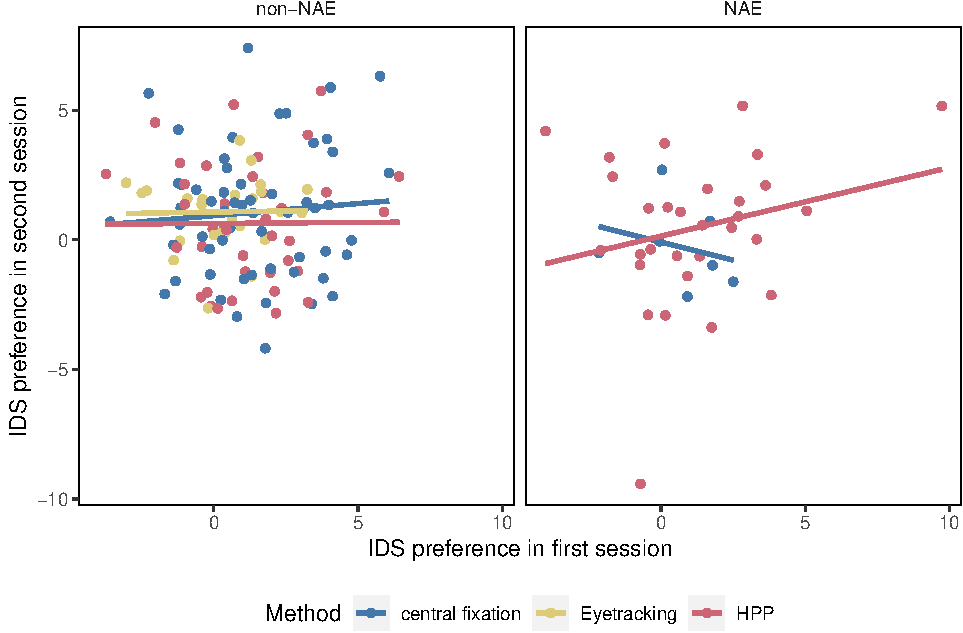
\includegraphics{MB1T_supplement_files/figure-latex/fig1-1.pdf}
\caption{\label{fig:fig1}Infants' preference in Session 1 and Session 2 with individual data points and regression lines color-coded by method (central fixation, eye-tracking, or HPP). Results are plotted separately for North American English-learning infants (right panel) and infants learning other languages and dialects (right panel).}
\end{figure}

NAE-learning infants showed greater IDS preferences than their non-NAE counterparts in MB1.
We therefore also assessed if test-retest reliability interacted with children's language background.
A linear mixed-effects model predicting IDS preference in Session 2 based on IDS preference in Session 1 (mean-centered), NAE (centered) and their interaction, including Lab as a random intercept, revealed no interaction, \(\beta\)=0.29, \emph{SE}=0.18, \emph{t}(151.30)=1.59, \emph{p}=.115 (Figure 1).

\hypertarget{s2.3.-participant-age}{%
\subsection{S2.3. Participant age}\label{s2.3.-participant-age}}

To investigate the possibility that age moderated test-retest reliability, we fit a linear mixed-effects model predicting predicting IDS preference in Session 2 from on IDS preference in Session 1 (mean-centered), participant age (mean-centered) and their interaction.
The model included a by-lab random intercept and a by-lab random slope for IDS preference in Session 1.
We found no evidence that age influenced test-retest reliability as indicated by the interaction between IDS preference in Session 1 and age, \(\beta\)=0.00, \emph{SE}=0.00, \emph{t}(76.60)=-0.85, \emph{p}=.398.

\newpage

\hypertarget{s3.-meta-analysis-of-test-retest-reliability}{%
\section{S3. Meta-analysis of test-retest reliability}\label{s3.-meta-analysis-of-test-retest-reliability}}

\begin{figure}
\centering
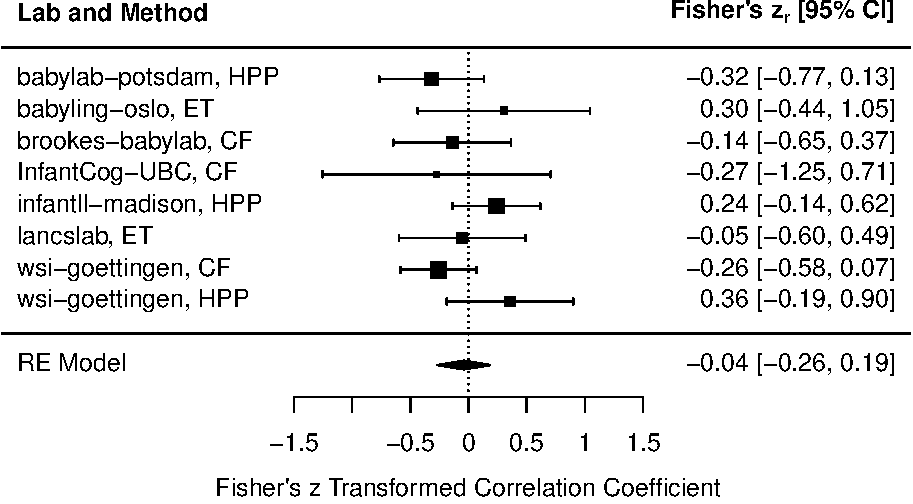
\includegraphics{MB1T_supplement_files/figure-latex/fig2-1.pdf}
\caption{\label{fig:fig2}Forest plot of test-retest reliability effect sizes. Each row represents Fisher's z transformed correlation coefficient and 95\% CI for a given lab and method (HPP = head-turn preference procedure; ET = eye-tracking; CF = central fixation). The black diamond represents the overall estimated effect size from the mixed-effects meta-analytic model.}
\end{figure}

In addition to the methods for assessing test-retest reliability reported in the main manuscript, we also investigated test-retest reliability across labs using a meta-analytic approach.
We used the metafor package (Viechtbauer, 2010) to fit a mixed-effects meta-analytic model on z-transformed correlations for each combination of lab and method using sample size weighting.
The model included random intercepts for lab and method.
The overall effect size estimate was not significantly different from zero, \emph{b} = -0.04, 95\% CI = {[}-0.26, 0.19{]}, \emph{p} = 0.73.
A forest plot of the effect sizes for each lab and method is shown in Figure 2.

\newpage

\hypertarget{s4.-alternative-dependent-variables}{%
\section{S4. Alternative Dependent Variables}\label{s4.-alternative-dependent-variables}}

To check the robustness of our results, we also investigated whether we obtained similar results with other possible dependent measures: average log-transformed looking times and a proportion-based preference measure. For each alternative dependent variable, we conducted the main analyses of test-retest reliability reported in the manuscript: the overall Pearson correlation, the test-retest linear mixed-effects model, and an inspection of applying stricter inclusion criteria for number of trials contributed.

\hypertarget{s4.1.-log-transformed-looking-times}{%
\subsection{S4.1. Log-transformed looking times}\label{s4.1.-log-transformed-looking-times}}

In these analyses, we calculated IDS preference by first log-transforming looking times for each trial, computing the average log-transformed looking time for IDS and ADS for each participant, and calculating the difference between average IDS and ADS log-transforming looking times.
We fit a linear mixed-effects model predicting IDS preference in Session 2 from IDS preference in Session 1, including a by-lab random intercept.
As in the analyses using average raw looking times, the results revealed no significant relationship between IDS preference in Session 1 and 2 (Table 1).
The Pearson correlation coefficient was also not statistically significant, \(r = .03\), 95\% CI \([-.12, .19]\), \(t(156) = 0.43\), \(p = .670\).
Applying successively stricter inclusion criteria --- by requiring a higher number of valid trials per condition in each session --- showed a similar pattern to the main manuscript, such that correlations increased somewhat with stricter inclusion criteria, but substantially reduced the sample size at the same time (Figure 3).

\begin{table}[tbp]

\begin{center}
\begin{threeparttable}

\caption{\label{tab:unnamed-chunk-7}Coefficient estimates from a linear mixed effects model predicting Log LT IDS preference in Session 2.}

\begin{tabular}{lllll}
\toprule
 & \multicolumn{1}{c}{Estimate} & \multicolumn{1}{c}{SE} & \multicolumn{1}{c}{t} & \multicolumn{1}{c}{p}\\
\midrule
Intercept & 0.14 & 0.07 & 2.05 & 0.09\\
Log LT IDS Preference Session 1 & -0.06 & 0.09 & -0.68 & 0.50\\
\bottomrule
\end{tabular}

\end{threeparttable}
\end{center}

\end{table}

\begin{figure}

{\centering 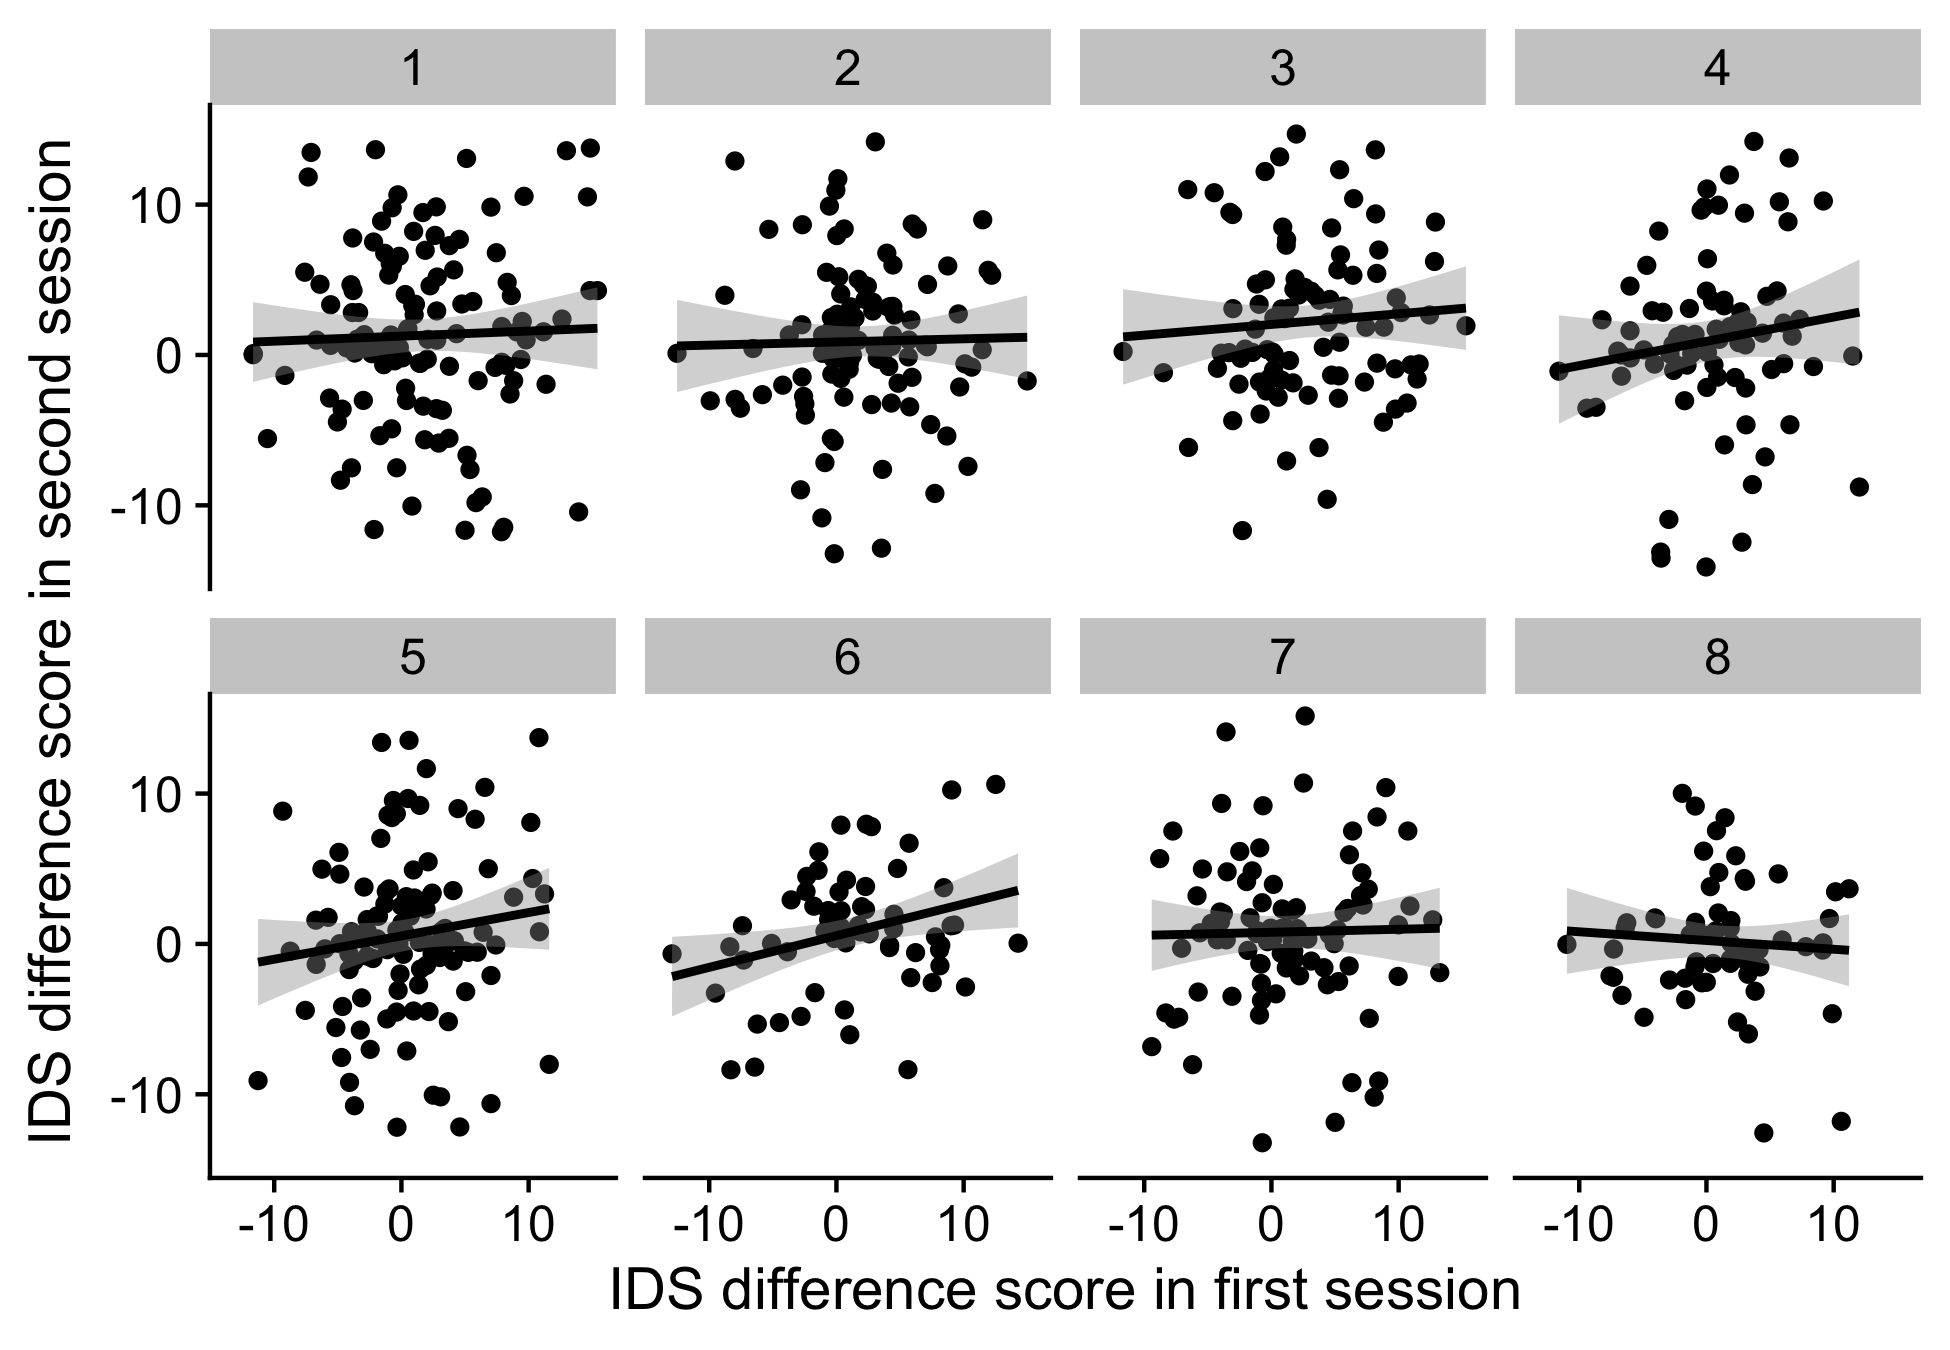
\includegraphics[width=5in]{MB1T_supplement_files/figure-latex/unnamed-chunk-8-1} 

}

\caption{IDS preferences (based on average log-looking times) of both sessions plotted against each other for each inclusion criterion. n indicates the number of included infants, r is the Pearson correlation coefficient as the indicator for reliability.}\label{fig:unnamed-chunk-8}
\end{figure}

\hypertarget{s4.2.-proportion-looking-to-ids}{%
\subsection{S4.2. Proportion looking to IDS}\label{s4.2.-proportion-looking-to-ids}}

\begin{table}[tbp]

\begin{center}
\begin{threeparttable}

\caption{\label{tab:unnamed-chunk-9}Coefficient estimates from a linear mixed effects model predicting IDS preference (based on proportion IDS looking) in Session 2.}

\begin{tabular}{lllll}
\toprule
 & \multicolumn{1}{c}{Estimate} & \multicolumn{1}{c}{SE} & \multicolumn{1}{c}{t} & \multicolumn{1}{c}{p}\\
\midrule
Intercept & 0.59 & 0.05 & 10.70 & 0.00\\
IDS Preference (proportion measure) Session 1 & -0.10 & 0.10 & -1.01 & 0.31\\
\bottomrule
\end{tabular}

\end{threeparttable}
\end{center}

\end{table}

Next, we calculated a proportion-based IDS preference measure by computing the average proportion (raw) looking time to IDS relative to total (raw) looking time to IDS and ADS for each subject (i.e., IDS looking time / (ADS looking time + IDS looking time)).
We fit a linear mixed-effects model predicting proportion-based IDS preference in Session 2 from propotion-based IDS preference in Session 1, including a by-lab random intercept.
As in the analyses using other measure of IDS preference, the results revealed no significant relationship between IDS preference in Session 1 and 2 (Table 2).
The Pearson correlation coefficient based on proportional IDS looking was also not statistically significant, \(r = .01\), 95\% CI \([-.15, .16]\), \(t(156) = 0.09\), \(p = .927\).
Stricter inclusion criteria increased the correlation somewhat, as in previous analyses (Figure 4).

\begin{figure}

{\centering 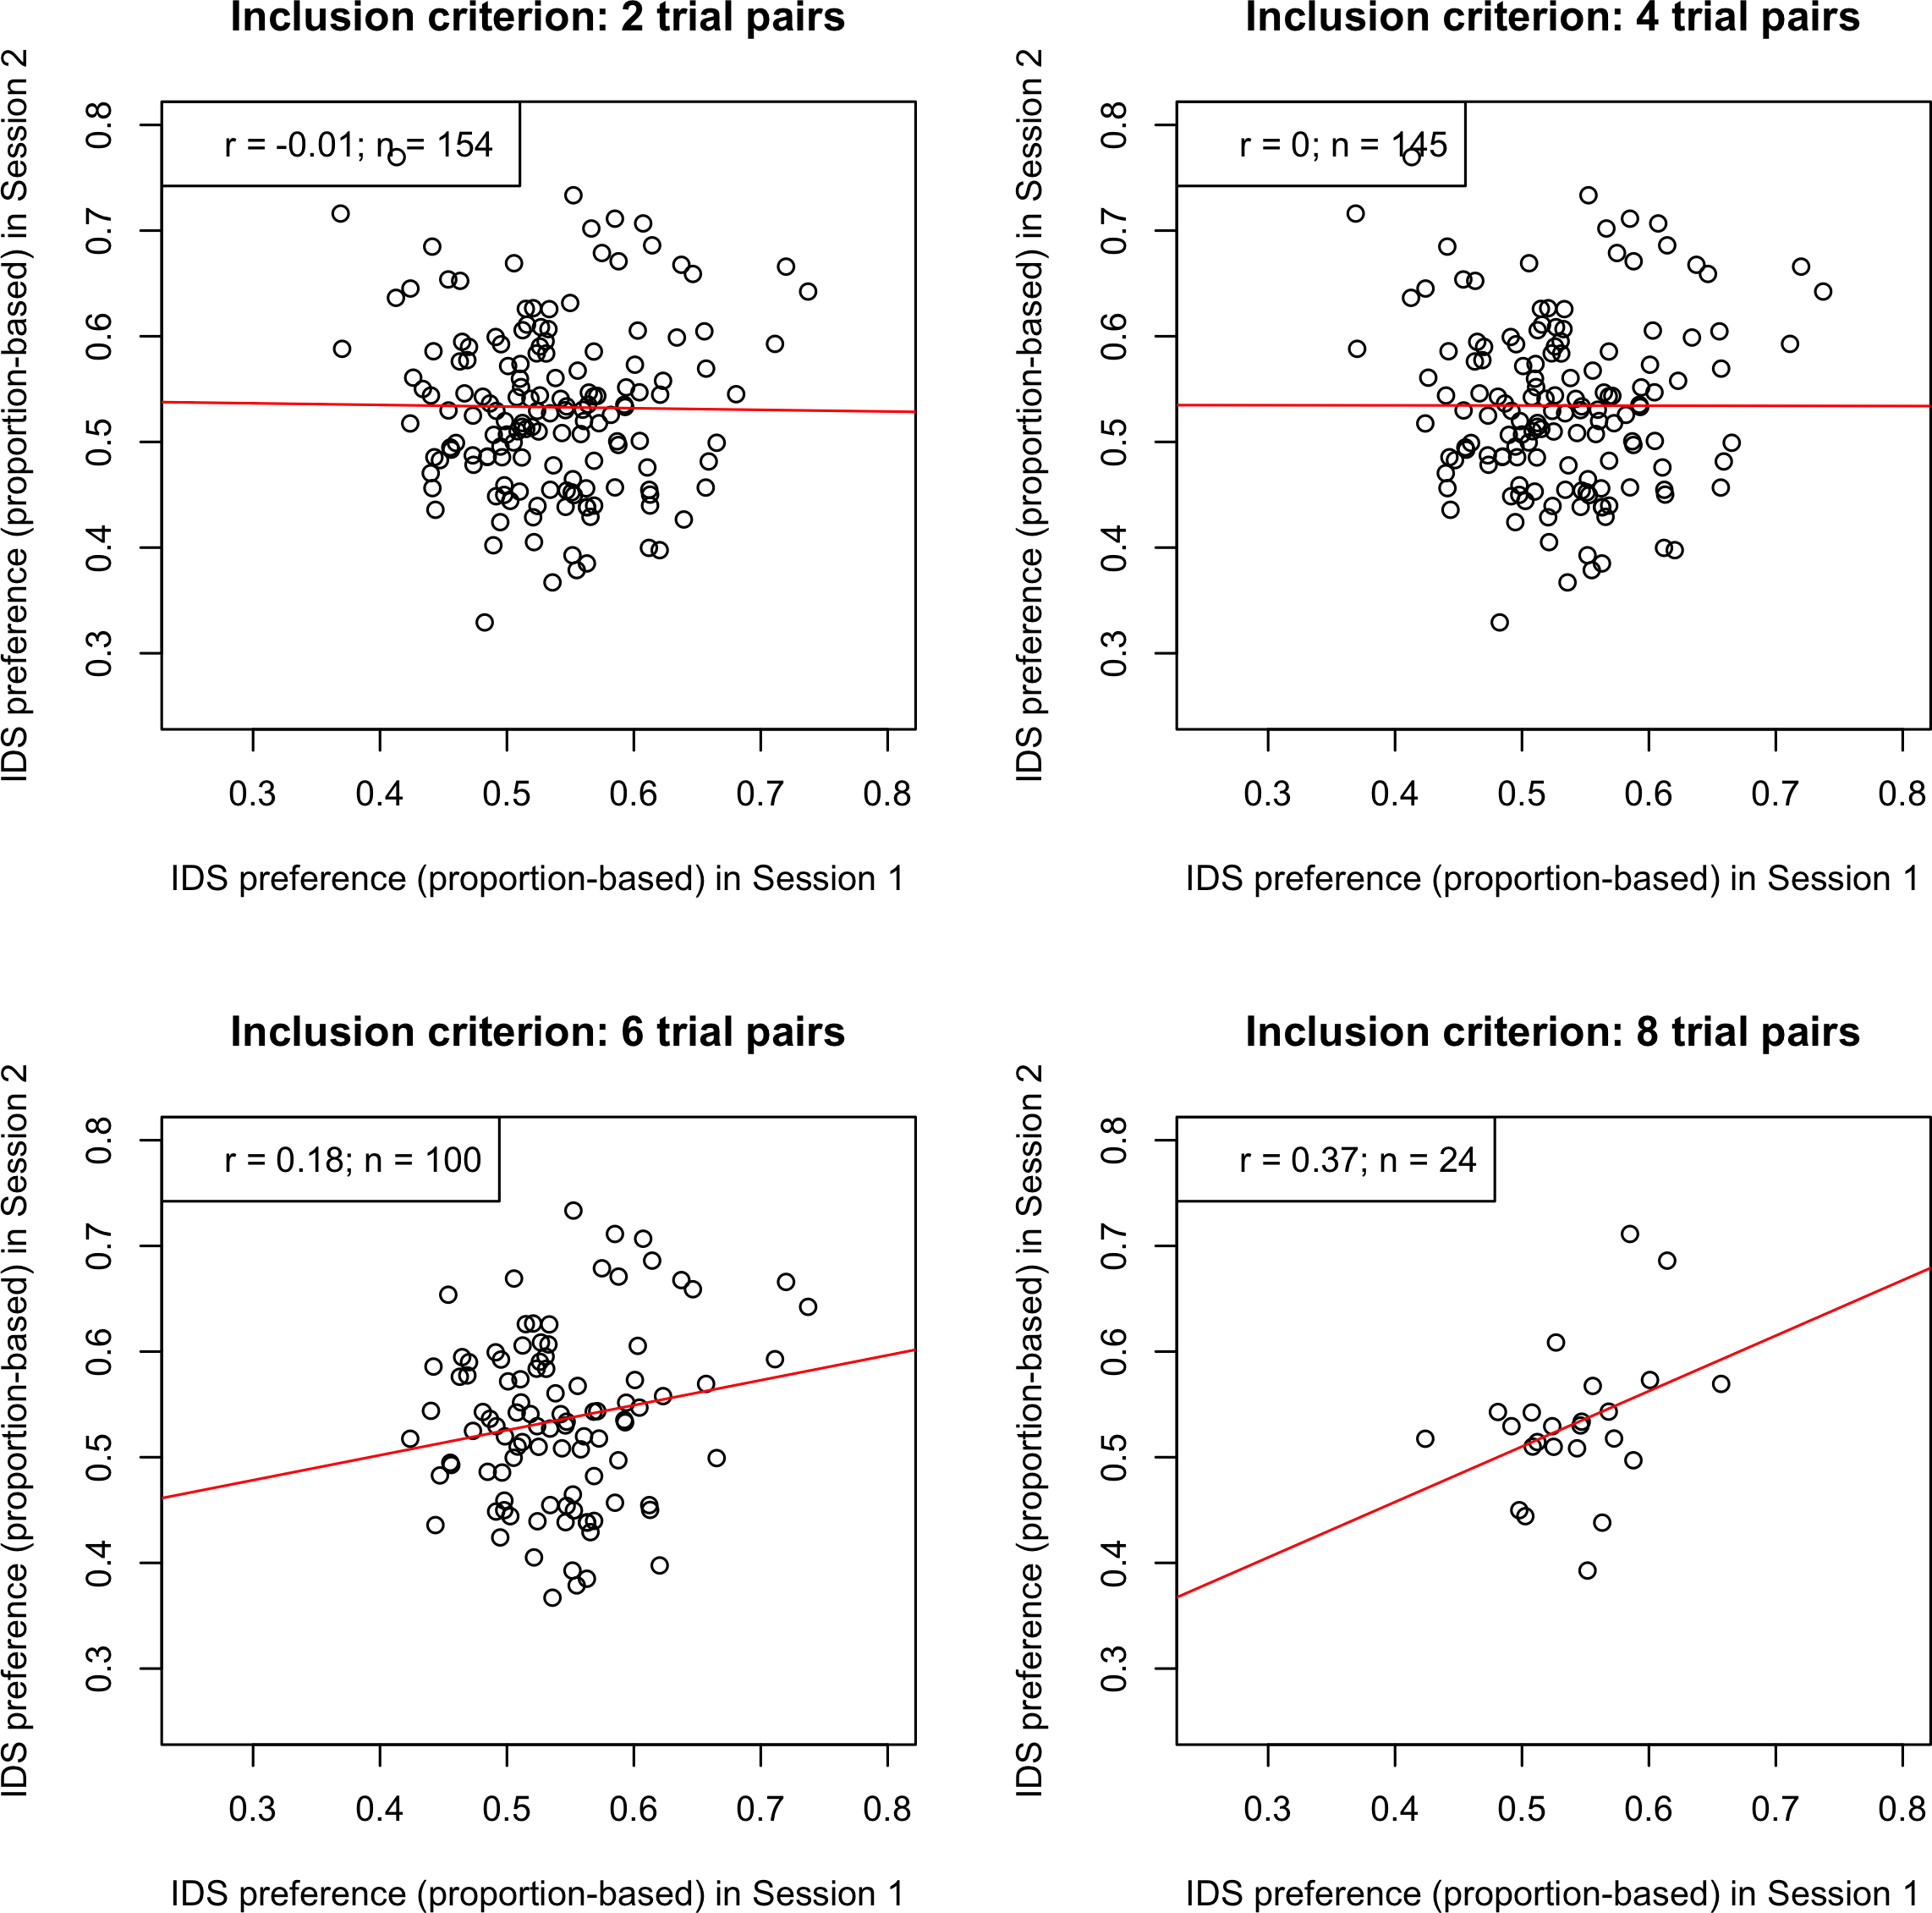
\includegraphics[width=5in]{MB1T_supplement_files/figure-latex/unnamed-chunk-11-1} 

}

\caption{IDS preferences (based on average log-looking times) of both sessions plotted against each other for each inclusion criterion. n indicates the number of included infants, r is the Pearson correlation coefficient as the indicator for reliability.}\label{fig:unnamed-chunk-11}
\end{figure}

\newpage

\hypertarget{s5.-sensitivity-of-test-retest-reliability-to-trial-number-inclusion-criteria}{%
\section{S5. Sensitivity of test-retest reliability to trial number inclusion criteria}\label{s5.-sensitivity-of-test-retest-reliability-to-trial-number-inclusion-criteria}}

To conduct a more fine-grained analysis of how stricter trial inclusion criteria affect test-retest reliability, we computed correlations while gradually increasing the number of total valid trials required for inclusion.
For this analysis, we required a minimum of 1 IDS and 1 ADS trial and gradually increased the number of total valid trials required in both sessions (irrespective of IDS and ADS condition) from 2 to 16 (the maximum number of total trials).
Figure 5 depicts the Pearson correlation coefficients for increasingly stricter requirements for the overall trial numbers of a given participant in both sessions.
Correlations only increase and reach conventional levels of significance once the number of total required trials for both sessions is greater than 12.

\begin{figure}
\centering
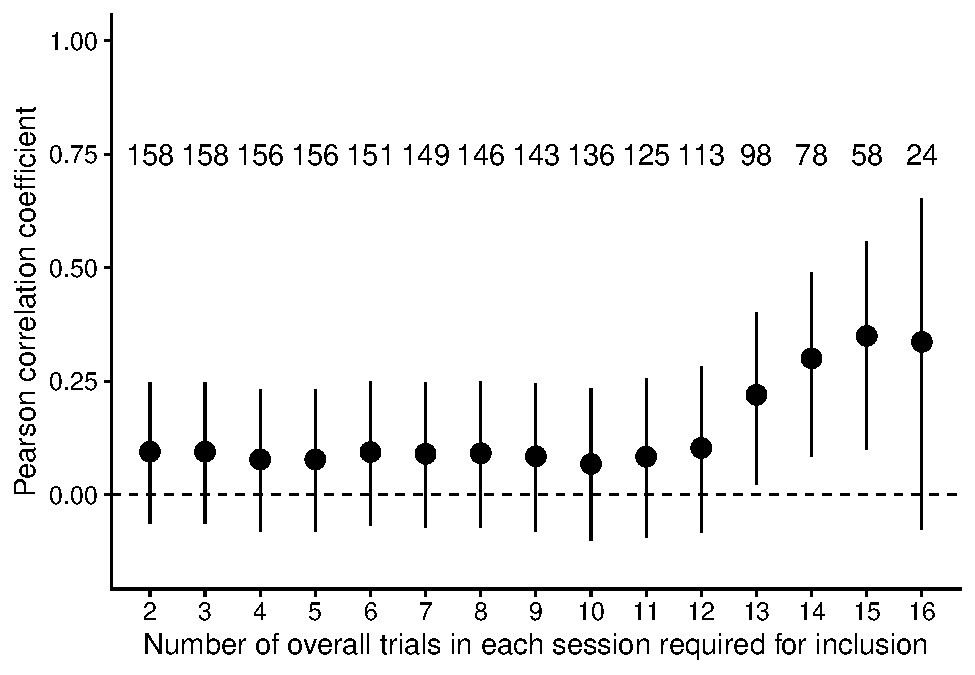
\includegraphics{MB1T_supplement_files/figure-latex/sfig5-1.pdf}
\caption{\label{fig:sfig5}Pearson correlation coefficient with increasingly strict trial-level inclusion criteria. The x-axis depicts the required number of overall valid trials in both session 1 and session 2. Dots represent corresponding correlation coefficients, with 95 percent CIs. The sample size is shown above each dot.}
\end{figure}

\hypertarget{s6.-patterns-of-preference-across-sessions}{%
\section{S6. Patterns of preference across sessions}\label{s6.-patterns-of-preference-across-sessions}}

We also conducted analyses to explore whether there were any patterns of preference reversal across test sessions.
While there was no strong correlation in the magnitude of IDS preference between test session 1 and test session 2, here we asked whether infants consistently expressed the same preference across test sessions.
Overall, 58.20\% of the infants had a consistent preference from test to retest session, indicating that infants were not more likely than chance to maintain their preference from test session 1 to test session 2 (exact binomial test; \emph{p} =
0.05).
Of the 158 total infants, 44.90\% of infants showed a consistent infant-directed speech preference and 13.30\% showed a consistent adult-directed speech preference.
23.40\% of infants switched from an infant-directed speech preference at test session 1 to an adult-directed speech preference at test session 2 and 18.40\% switched from an adult-directed speech preference to an infant-directed speech preference.

Next, we explored whether we could detect any systematic clustering of infants with distinct patterns of preference across the test and retest session.
We took a bottom-up approach and conducted a \emph{k}-means clustering of the test-retest difference data (here using log-transformed looking time data).
We found little evidence of distinct clusters emerging from these groupings: the clusterings ranging from \emph{k}=2 (2 clusters) to \emph{k}=4 (4 clusters) appear to mainly track whether participants are approximately above or below the mean looking time difference for test session 1 and test session 2 (Figure 6A).
The diagnostic elbow plot shows little evidence of a qualitative improvement as the number of clusters is increased, which suggests little evidence for a distinctive set of clusters of participants who showed similar patterns of looking across the test and retest sessions (Figure 6B).

\begin{figure}
\centering
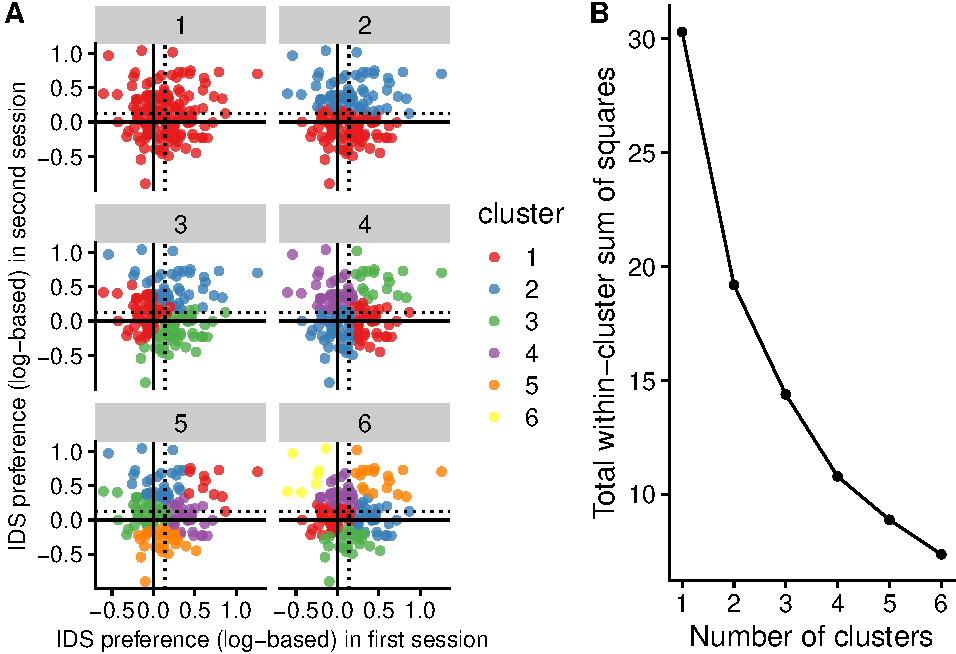
\includegraphics{MB1T_supplement_files/figure-latex/fig6-1.pdf}
\caption{\label{fig:fig6} (A) Results from the k-means clustering analysis of IDS preference (based on average log looking times) in session 1 and 2 for different numbers of k and (B) the corresponding elbow plot of the total within-cluster sum of squares. In (A), points represent indvidual participants' magnitude of looking time difference at test sessions 1 (x-axis) and 2 (y-axis). The solid line indicates no preference for IDS vs.~ADS, the dotted lines indicate mean IDS preference at test session 1 and 2, respectively. Colors indicate clusters from the k-means clustering for different values of k.}
\end{figure}

\hypertarget{s7.-relationship-between-number-of-contributed-trials-in-each-session}{%
\section{S7. Relationship between number of contributed trials in each session}\label{s7.-relationship-between-number-of-contributed-trials-in-each-session}}

\begin{figure}
\centering
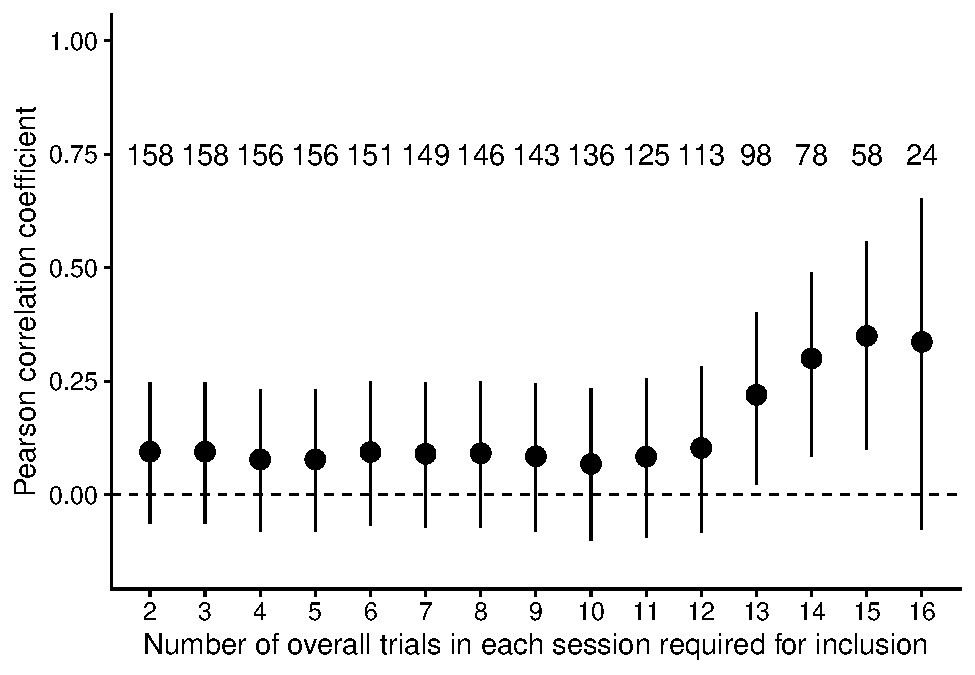
\includegraphics{MB1T_supplement_files/figure-latex/sfig7-1.pdf}
\caption{\label{fig:sfig7}Correlation between the number of trials contributed in session 1 and session 2. Each data point represents one infant. Colored lines represent linear fits for each method.}
\end{figure}

Are there stable individual differences in how likely an infant is to contribute a high number of trials?
To answer this question, we conducted an exploratory analysis investigating whether there is a relationship between the number of trials an infant contributed in session 1 and session 2.
Do infants who contribute a higher number of trials during their first testing session also tend to contribute more trials during their second testing session?
A positive correlation between trial numbers during the first and second session would indicate that their is some stability in a given infants' likelihood of remaining attentive throughout the experiment.
On the other hand, the absence of a correlation would indicate that the number of trials a given infant contributes is not predictive of how many trials they might contribute during their next session.

We found a strong positive correlation between number of trials contributed during the first and the second session \(r = .58\), 95\% CI \([.47, .68]\), \(t(159) = 9.05\), \(p < .001\) (Figure 7).
This result suggests that if infants contribute a higher number of trials in one session, compared to other infants, they are likely to contribute a higher number of trials in their next session.
This finding is consistent with the hypothesis that how attentive infants are throughout an experiment (and hence how many trials they contribute) is a stable individual difference, at least for some infant looking time tasks.
Researchers should therefore be mindful of the fact that decisions about including or excluding infants based on trials contributed may selectively sample a specific sub-set of the infant population they are studying (Byers-Heinlein, Bergmann, \& Savalei, 2021; DeBolt, Rhemtulla, \& Oakes, 2020).

\hypertarget{s8.-correlations-in-average-looking-times-between-sessions}{%
\section{S8. Correlations in average looking times between sessions}\label{s8.-correlations-in-average-looking-times-between-sessions}}

To what extent are participants looking times between the two sessions related?
To test this question, we first investigated whether participants' overall looking times --- irrespective of condition --- were correlated between the first and second session.
There was a robust correlation between average looking time in Session 1 and Session 2: infants with longer looking times during their first session also tended to look longer during their second session, \(r = .45\), 95\% CI \([.31, .57]\), \(t(156) = 6.28\), \(p < .001\).
This relationship held even after controlling for number of trials in the first and second session, suggesting that the relationship in between average looking could not be entirely explained by correlation between number of trials contributed between the two sessions (S7), \(b = 0.42\), 95\% CI \([0.27, 0.58]\), \(t(154) = 5.52\), \(p < .001\) (Figure 8A).

Next, we explored the extent to which average looking times for IDS and ADS stimuli specifically were related.
First, we found similar correlations in average looking time to IDS stimuli in Session 1 and 2 (\(r = .38\), 95\% CI \([.24, .51]\), \(t(156) = 5.19\), \(p < .001\); Figure 8B) and ADS stimuli in Session 1 and 2 (\(r = .40\), 95\% CI \([.26, .53]\), \(t(156) = 5.49\), \(p < .001\)).
To test whether these correlations were specific to looking times for IDS or ADS stimuli alone, we fit linear regression models predicting average looking to IDS (or ADS) stimuli in Session 2 from average looking to IDS and ADS stimuli in Session 1.
We found that average looking to IDS stimuli in Session 2 could be predicted from average looking to IDS stimuli in Session 1, even after controlling for average looking to ADS stimuli in Session 1, \(b = 0.21\), 95\% CI \([0.01, 0.41]\), \(t(155) = 2.11\), \(p = .037\).
Conversely, average looking to ADS stimuli in Session 2 could be predicted from average looking to ADS stimuli in Session 1, even after controlling for average looking to IDS stimuli in Session 1, \(b = 0.36\), 95\% CI \([0.14, 0.58]\), \(t(155) = 3.20\), \(p = .002\).
These results suggest that the condition-specific correlations in average looking time cannot be fully explained by the fact that infants' overall looking times between sessions are correlated.

Finally, we inspected item-level correlations between the two test sessions.
Specifically, we investigated the relation between items composed of the same recording clips in Session 1 and Session 2 (but with a reversed order of clips between the two sessions).
We fit a linear mixed-effects model predicting item-level looking time in Session 2 from item-level looking time in Session 1, including random intercepts for participant, item, and lab, as well as an random slope for item-level looking time in Session 1 for participant and lab.
Item-level looking in Session 2 was related to item-level looking in Session 1, \(\hat{\beta} = 0.17\), 95\% CI \([0.07, 0.27]\), \(t(5.52) = 3.38\), \(p = .017\) (Figure 8C).
Similar results hold if looking times are log-transformed

\begin{figure}

{\centering 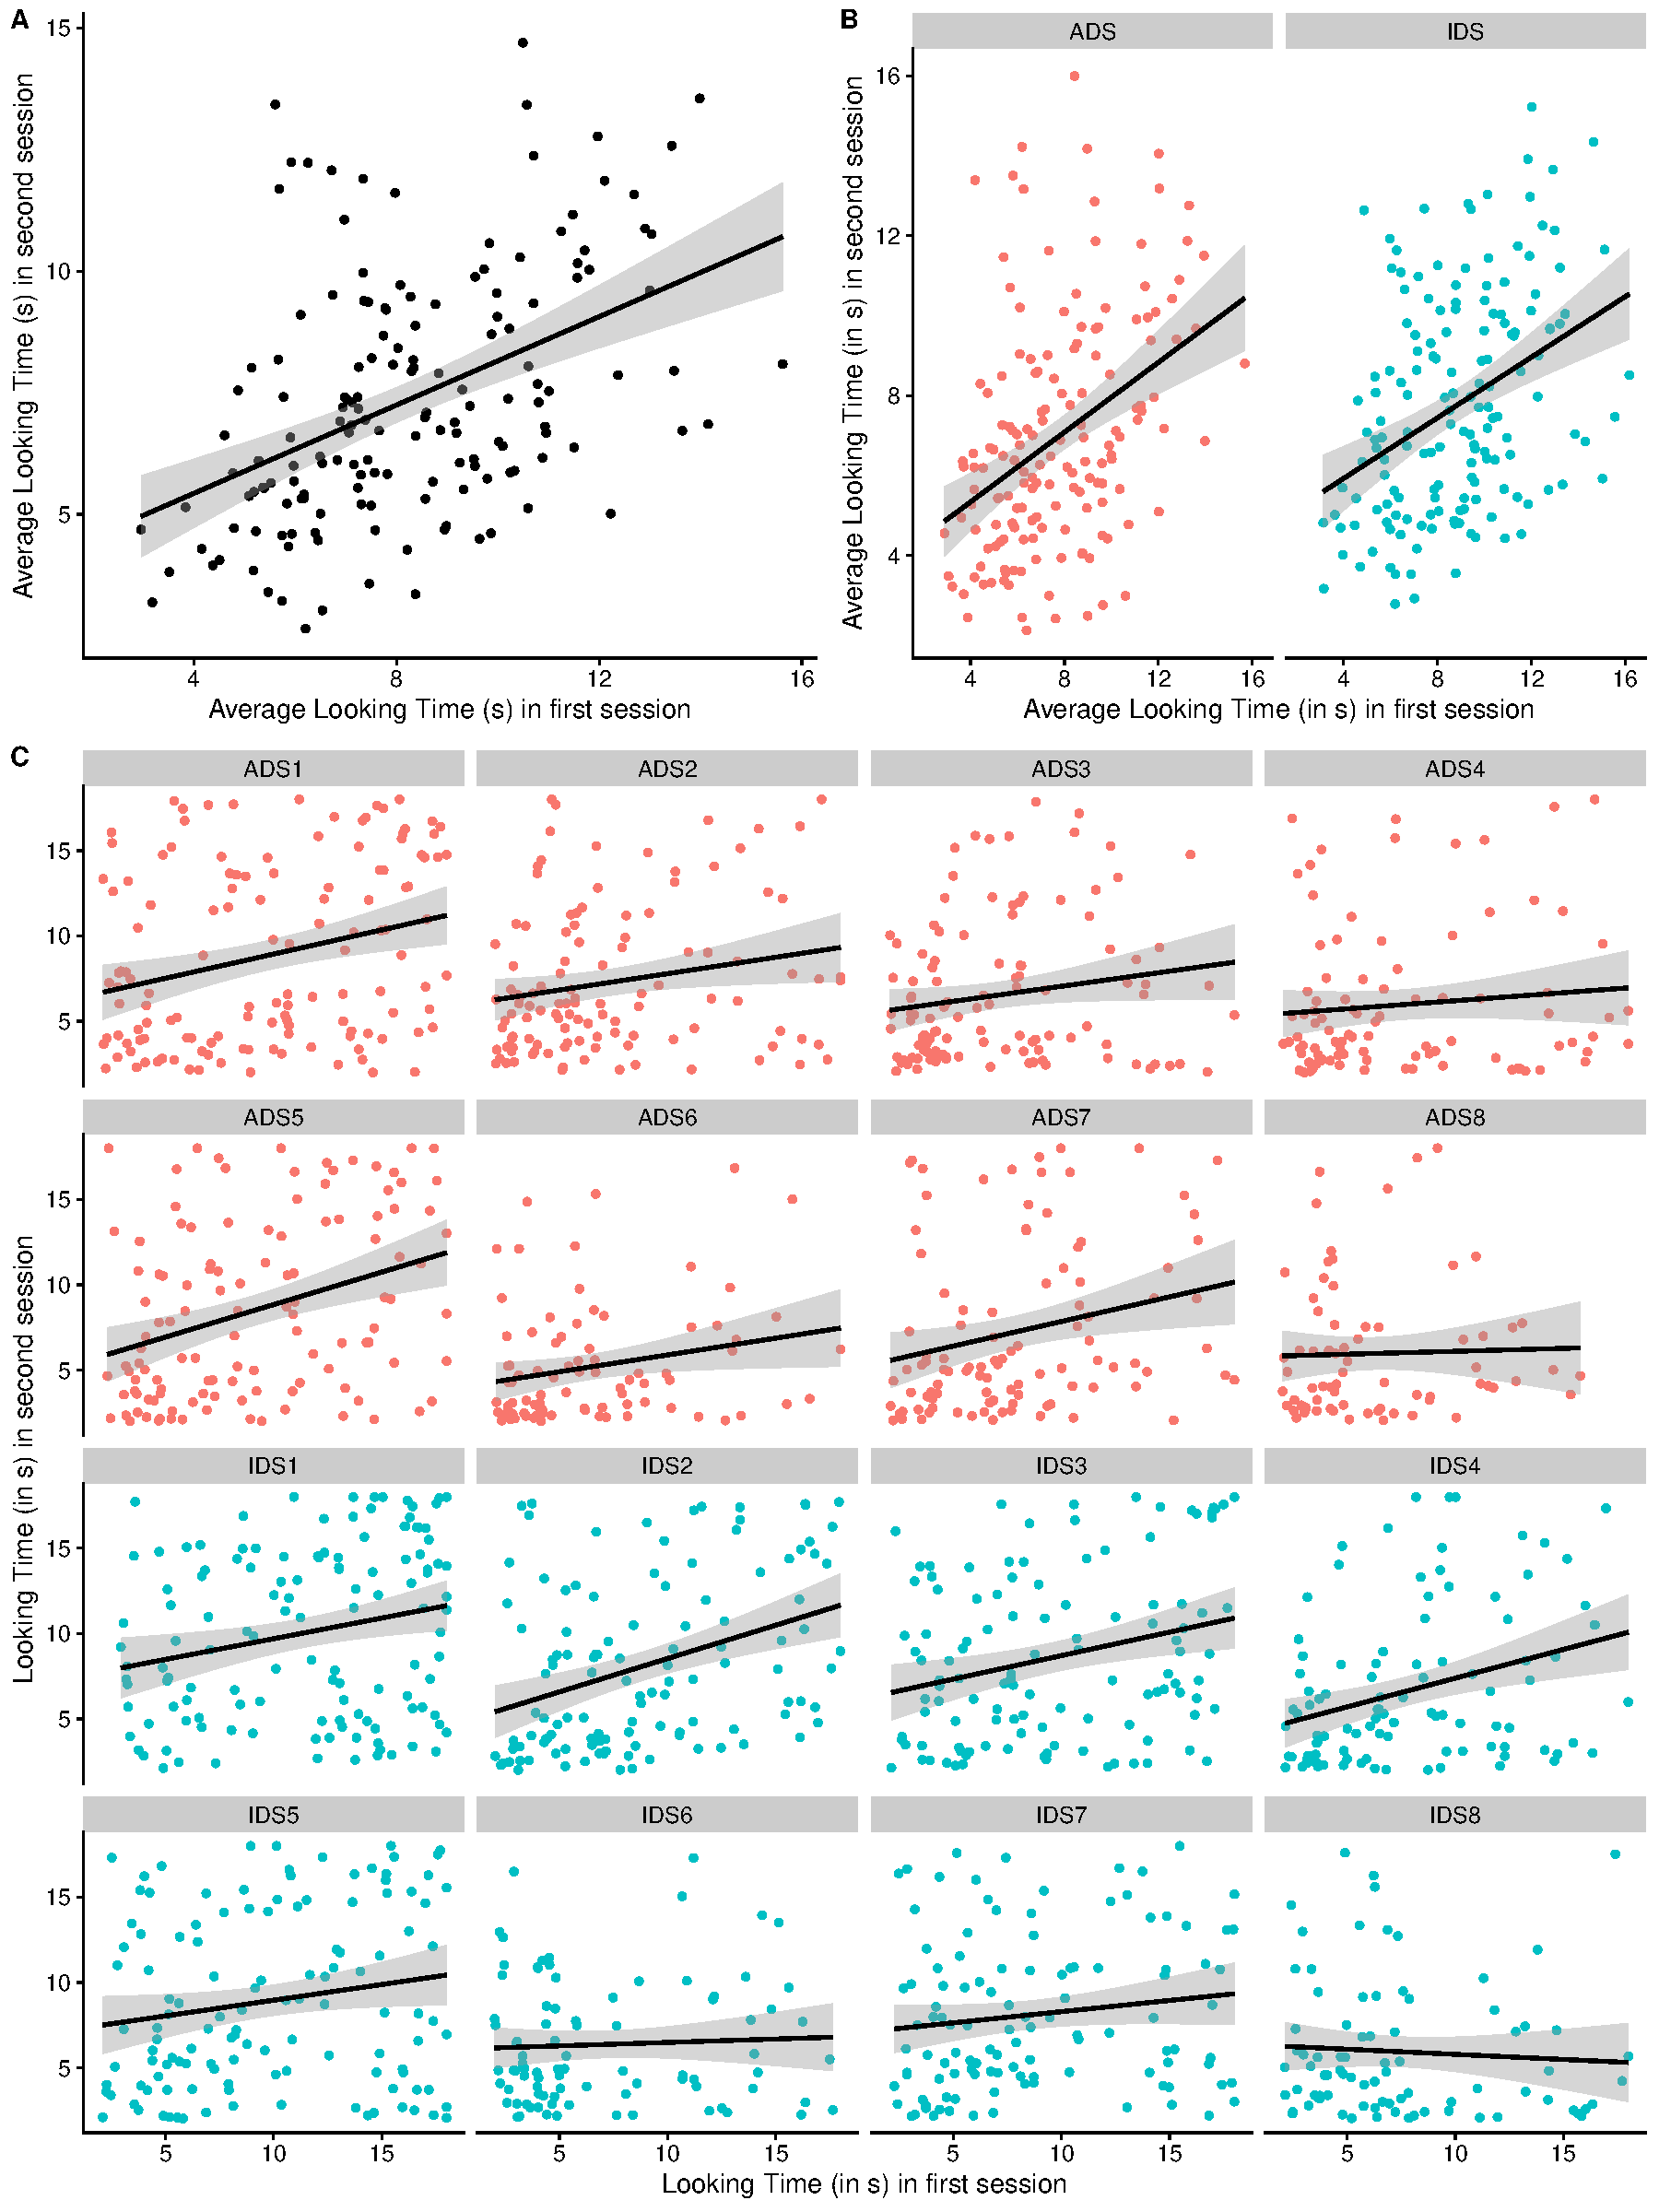
\includegraphics{MB1T_supplement_files/figure-latex/sfig8-1} 

}

\caption{Correlations in average looking time (in ms) between Session 1 and 2 (A) overall, (B) by condition, and (C) by item.}\label{fig:sfig8}
\end{figure}

\hypertarget{s9.-by-item-pair-preference-scores-across-sessions}{%
\section{S9. By-item-pair preference scores across sessions}\label{s9.-by-item-pair-preference-scores-across-sessions}}

\begin{table}[tbp]

\begin{center}
\begin{threeparttable}

\caption{\label{tab:unnamed-chunk-19}Mixed-effects model results predicting IDS preference during session 1 from IDS preference at session 2 at the stimulus level.}

\begin{tabular}{llllll}
\toprule
Term & \multicolumn{1}{c}{$\hat{\beta}$} & \multicolumn{1}{c}{95\% CI} & \multicolumn{1}{c}{$t$} & \multicolumn{1}{c}{$\mathit{df}$} & \multicolumn{1}{c}{$p$}\\
\midrule
Intercept & 1.02 & {}[0.14, 1.90] & 2.27 & 6.55 & .060\\
Diff 1 & 0.07 & {}[-0.01, 0.14] & 1.79 & 718.46 & .074\\
\bottomrule
\end{tabular}

\end{threeparttable}
\end{center}

\end{table}

Finally, we inspected on a more fine-grained item-level whether IDS preference in Session 1 was related to IDS preference in Session 2.
To do so, we exploited the fact the specific IDS and ADS stimuli were paired together in test orders in both sessions, such that one IDS stimulus (e.g., IDS1) always occurred adjacently to a specific ADS stimulus (e.g., ADS1).
We therefore computed stimulus-specific IDS preference scores by calculating the difference in raw looking time for each of the eight IDS-ADS stimulus pairs for each participant (when both trials in a given pair were available).
We then fit a linear mixed-effects model predicting stimulus-specific IDS preference in Session 2 from stimulus-specific IDS preference in Session 1, including by-participant and by-lab random intercepts (models with more complex random effects structure, including by-item random effects, failed to converge).
There was a marginal, but non-significant relation in stimulus-specific IDS preference between the two test sessions (Table 3).

\newpage

\hypertarget{references}{%
\section{References}\label{references}}

\begingroup
\setlength{\parindent}{-0.5in}
\setlength{\leftskip}{0.5in}

\hypertarget{refs}{}
\begin{CSLReferences}{1}{0}
\leavevmode\vadjust pre{\hypertarget{ref-byers2021six}{}}%
Byers-Heinlein, K., Bergmann, C., \& Savalei, V. (2021). Six solutions for more reliable infant research. \emph{Infant and Child Development}, e2296.

\leavevmode\vadjust pre{\hypertarget{ref-debolt2020robust}{}}%
DeBolt, M. C., Rhemtulla, M., \& Oakes, L. M. (2020). Robust data and power in infant research: A case study of the effect of number of infants and number of trials in visual preference procedures. \emph{Infancy}, \emph{25}(4), 393--419.

\leavevmode\vadjust pre{\hypertarget{ref-manybabies2020quantifying}{}}%
ManyBabies Consortium. (2020). Quantifying sources of variability in infancy research using the infant-directed-speech preference. \emph{Advances in Methods and Practices in Psychological Science}, \emph{3}(1), 24--52.

\leavevmode\vadjust pre{\hypertarget{ref-R-metafor}{}}%
Viechtbauer, W. (2010). Conducting meta-analyses in {R} with the {metafor} package. \emph{Journal of Statistical Software}, \emph{36}(3), 1--48. Retrieved from \url{https://doi.org/10.18637/jss.v036.i03}

\end{CSLReferences}

\endgroup


\end{document}
